\documentclass[3p,12pt]{elsarticle}

\usepackage{amssymb}
\usepackage{amsmath}
\usepackage{float}
\usepackage{subcaption}
\usepackage{booktabs}
\usepackage{etoolbox}
\AtBeginEnvironment{tabular}{\def\baselinestretch{1}\selectfont}
\usepackage[section]{placeins}
\pretocmd{\subsection}{\FloatBarrier}{}{}
\renewcommand{\topfraction}{0.90}
\renewcommand{\bottomfraction}{0.70}
\renewcommand{\textfraction}{0.10}
\renewcommand{\floatpagefraction}{0.75}
\emergencystretch=3em

\newcommand{\MITgcm}{\textsc{MITgcm}}
\newcommand{\FNO}{FNO}

\begin{document}

\begin{frontmatter}

\title{An adjoint-faithful Fourier neural operator for a double-gyre ocean:\\ progress summary}

\author[ucsb]{Maxime Jalabert}
\ead{mjalabert@ucsb.edu}
\author[jpl]{Ian Fenty}
\author[jpl]{Ou Wang}

\affiliation[ucsb]{organization={University of California, Santa Barbara}}
\affiliation[jpl]{organization={NASA Jet Propulsion Laboratory}}

\begin{abstract}
This note summarizes progress, as of 25 August 2026, on training a Fourier neural
operator (\FNO) emulator of a \MITgcm{} double-gyre configuration whose
tangent-linear and adjoint sensitivities match the ocean model's, not only its
forecast trajectories. A 27.3-million-parameter, one-input/one-output \FNO{} was
trained from scratch on a weakly turbulent regime (S0) and then fine-tuned for a
short second stage at a longer autoregressive horizon; the fine-tune improves
essentially every forward forecast metric without trading away short-horizon
skill. A preliminary adjoint comparison against a \MITgcm{}/TAF ground-truth
sensitivity map, however, finds that the trained emulator's reverse-mode gradient
is a poor match to the true adjoint: near-zero pattern correlation and amplitude
errors of six- to thirty-eight-fold at leads of 10--90 days, concentrated in
Jacobian error rather than trajectory drift. This finding motivates the
adjoint-faithful training study now underway, which adds a forward
perturbation-response term to the training objective without ever exposing the
model to an adjoint value during training or selection. The response-data
generation infrastructure and its integrity gates are built and passing; model
training has not yet started.
\end{abstract}

\end{frontmatter}

\section{The production forward emulator}
\label{sec:emulator}

\subsection{Architecture and state}

The overall map, state convention, and Fourier-operator backbone follow the FNO
ocean-emulation architecture of Bire et al.~\cite{Bire2025}, who developed and
validated this class of emulator for the double gyre at $0.25^\circ\times0.25^\circ$
resolution; the model described here adapts it to a one-input Markov map at
one-degree resolution with the per-mode spectral normalization described below.
The emulator is a single Markov operator $F_\theta:[x_t,S]\to x_{t+10}$ predicting
the full 46-channel prognostic state ten days ahead on the \MITgcm{}
\texttt{tutorial\_baroclinic\_gyre} configuration (62$\times$62, one degree):
fifteen vertical levels each of zonal velocity $U$, meridional velocity $V$ and
potential temperature $\Theta$, plus the free surface $\eta$. Five physical
static channels (wind stress, wet mask, Coriolis parameter, grid spacing, SST
relaxation target) and a two-channel sine/cosine position encoding are appended,
for 53 lifted input channels. The state is deliberately kept closed --- all
fifteen levels of $U$, $V$, $\Theta$, plus $\eta$ --- so that the map is a
self-contained prognostic operator whose Jacobian can serve as a tangent/adjoint
operator, which a reduced state would not support.

The network is a three-block Fourier neural operator, 32$\times$32 retained
Fourier modes, hidden width 128, with a parallel bias-free $3\times3$ local
correction and six pointwise channel LayerNorms, 27{,}297{,}960 parameters in
total (Table~\ref{tab:arch}). Inside each spectral convolution the per-mode
channel-mixing matrix is capped to unit spectral norm by two power iterations
per forward pass~\cite{McCabe2023}, one-sided so that a mode already below the cap is left
untouched and carries no gradient. The cap bounds one constituent of the block,
not the full block Jacobian, so legitimate transient amplification through the
skip connections, channel MLP and local branch remains representable.

\begin{table}[H]
\centering
\begin{tabular}{ll}
\toprule
Item & Value \\
\midrule
Grid / interval & $62\times62$, $\Delta t=10$ days, direct state (not residual) \\
Fourier modes & $32\times32$ \\
Hidden width & 128 \\
FNO blocks & 3 \\
Local branch & bias-free $3\times3$, zero-initialized \\
Spectral normalization & per-mode $\sigma_{\max}\le1$, 1{,}632 modes, materialized at write \\
Parameters & 27{,}297{,}960 (97.95\% in the spectral convolutions) \\
\bottomrule
\end{tabular}
\caption{Core architecture of the production \FNO{}, identical between the
parent and the fine-tuned child.}
\label{tab:arch}
\end{table}

\subsection{Training, validation and inference}

The \emph{parent}, \texttt{model\_c\_production\_1in\_1out\_spectralnorm\_v1},
is trained from random initialization with an eight-term, fully dimensionless
objective (state, increment, autoregressive rollout, spectral, boundary,
pressure-gradient, continuity, barotropic-transport terms) on a six-call,
60-day autonomous rollout, 7{,}680 Adam steps --- each step one optimizer
update computed from an effective batch of eight 60-day training sequences ---
3.21~h on one V100. The \emph{child}, \texttt{..\_ft90\_v1}, is a short second
stage --- initialized from the parent, otherwise identical architecture,
normalizer, and objective --- extended to a nine-call, 90-day rollout at a
constant, five-times-lower learning rate for 1{,}920 steps (37.5\% of the
parent's exposure, 1.67~h). Every checkpoint is autoregressed 360 days from
102 pooled validation starts (34 evenly spaced starts in each of the three
wind regimes S0/S1/S2) and selected by a rule with three requirements:
short-horizon skill within 5\% of the best candidate in every field; a bounded
twin-perturbation growth rate (defined below); and, among the checkpoints
meeting both, the smallest degradation of 90--360-day error relative to a
train-only climatology baseline. Held inference uses 15 fixed S0 starts,
never used for training or selection, autoregressed to day 2{,}000 against
lead-matched \MITgcm{} truth.

The growth rate is measured entirely within the trained \FNO{}: its own
initial state is perturbed by a small (1\%) relative amount, and both the
perturbed and unperturbed states are autoregressed through the \emph{trained
emulator itself}, with no \MITgcm{} run at all, for 200 ten-day calls. Fitting
the exponential rate at which the two trajectories separate over the later
calls gives one number per checkpoint, capped at $\le1$ per call, so a
checkpoint whose own repeated map would amplify small differences into a
runaway drift over a 2{,}000-day rollout is rejected before it ever reaches
held inference. This is a different question from the adjoint comparison in
Section~\ref{sec:adjoint}. The growth rate asks only whether the trained
\FNO{}'s own nonlinear dynamics are self-consistently bounded when compared
against themselves, iterated many times; it never involves \MITgcm{} and says
nothing about whether any single derivative of the emulator is physically
correct. The adjoint study instead asks whether the \emph{exact, infinitesimal}
derivative of that same trained \FNO{}, computed once by reverse-mode
differentiation at a given lead, structurally matches \MITgcm{}'s true
derivative at the same point. A checkpoint can pass the first test and fail
the second, and Section~\ref{sec:adjoint} shows that this is exactly what
happens here: bounded, well-behaved own-dynamics do not imply a physically
correct Jacobian.

\subsection{Key results}

The fine-tune improves nearly every measured quantity relative to the parent,
without the usual short-horizon trade-off (Table~\ref{tab:results}). Figures
\ref{fig:fig8} and \ref{fig:fig7a} show the pooled 15-member held inference
through day 2{,}000 and the day-60/day-2{,}000 streamfunction anomaly for both
models.

\begin{table}[H]
\centering
\small
\begin{tabular}{lrr}
\toprule
Metric & Parent & Fine-tuned (ft90) \\
\midrule
10--90 d RMSE-AUC, surface pressure & 0.579 & \textbf{0.267} \\
Day-2{,}000 RMSE / climatology, SST & 1.425 (worse) & \textbf{0.924} (better) \\
Day-2{,}000 RMSE / climatology, pressure & 0.478 & \textbf{0.248} \\
Western boundary / interior anomaly ratio (truth 23.1) & 5.06 & \textbf{8.16} \\
Max. normalized amplitude through day 2{,}000 (target $\le8$) & 10.33 & 8.43 \\
Twin-perturbation growth rate per call (target $\le1$) & 1.0132 & 1.0083 \\
\bottomrule
\end{tabular}
\caption{Headline forward results, parent versus fine-tuned child, 15-member S0
held inference. Both still fail the declared day-2{,}000 amplitude and growth-rate
gates; the fine-tune moves substantially toward them without reaching them.}
\label{tab:results}
\end{table}

Table~\ref{tab:results} reads consistently in one direction: the fine-tune
improves every entry. RMSE-AUC is the area under the RMSE-versus-lead-time
curve over the stated window (10--90 days here) rather than the error at a
single lead, so a lower value means uniformly better skill across the whole
horizon, not just a better score on one particular day. The western
boundary/interior anomaly ratio compares the day-2{,}000 streamfunction
anomaly in the four-cell-wide western boundary band to the same quantity
averaged over the interior; \MITgcm{}'s value of 23.1 shows its transient
anomaly is far more concentrated in the western boundary current than either
emulator reproduces. Both models remain well short of that concentration,
though the fine-tune raises the ratio from 5.06 to 8.16 --- about 1.6 times
the parent's value. The last two rows are the acceptance ceilings adopted for
this project, and both are worst-case, not average-case, statistics. The
normalized amplitude is measured in the same pointwise-normalized
(z-score) coordinates the network is trained in: at every ten-day lead of
every one of the 15 held-inference members, take the single largest absolute
value across all 46 channels and all wet grid cells, then keep the largest
such value over the whole 2{,}000-day rollout. A value of 8 means that,
somewhere in space, in some channel, at some point in some member's
trajectory, the state reached eight training-climatology standard deviations
from its pointwise mean; the target $\le8$ caps that single worst excursion
before the rollout is judged to have drifted into an unphysical regime, not
the typical error level. The growth rate is the same twin-perturbation
diagnostic described in Section~\ref{sec:emulator}, here reported as the
worst value obtained from several independent validation starts rather than
their average; the target $\le1$ requires even the least favorable starting
state to show no net amplification. Both models still exceed both ceilings,
which is why day-2{,}000 behavior remains an open problem even though every
other entry in the table improves.

\begin{figure}[htbp]
\centering
\begin{subfigure}[t]{0.48\textwidth}
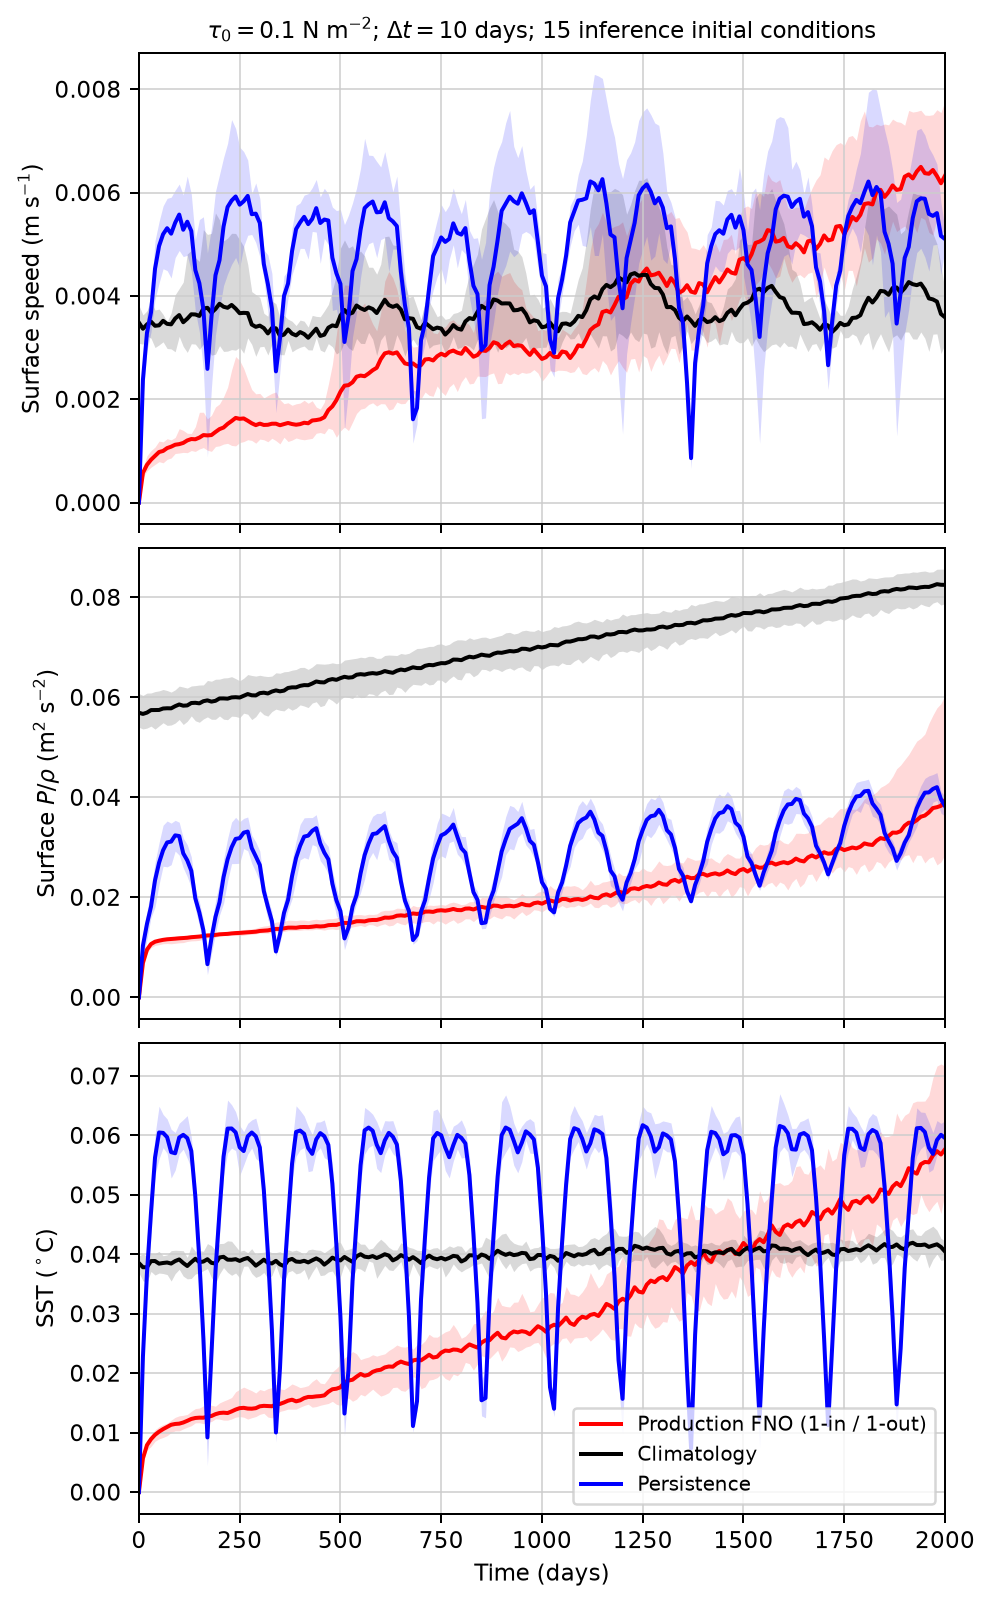
\includegraphics[width=\textwidth]{figures/parent_figure8_rmse.png}
\caption{Parent}
\end{subfigure}
\hfill
\begin{subfigure}[t]{0.48\textwidth}
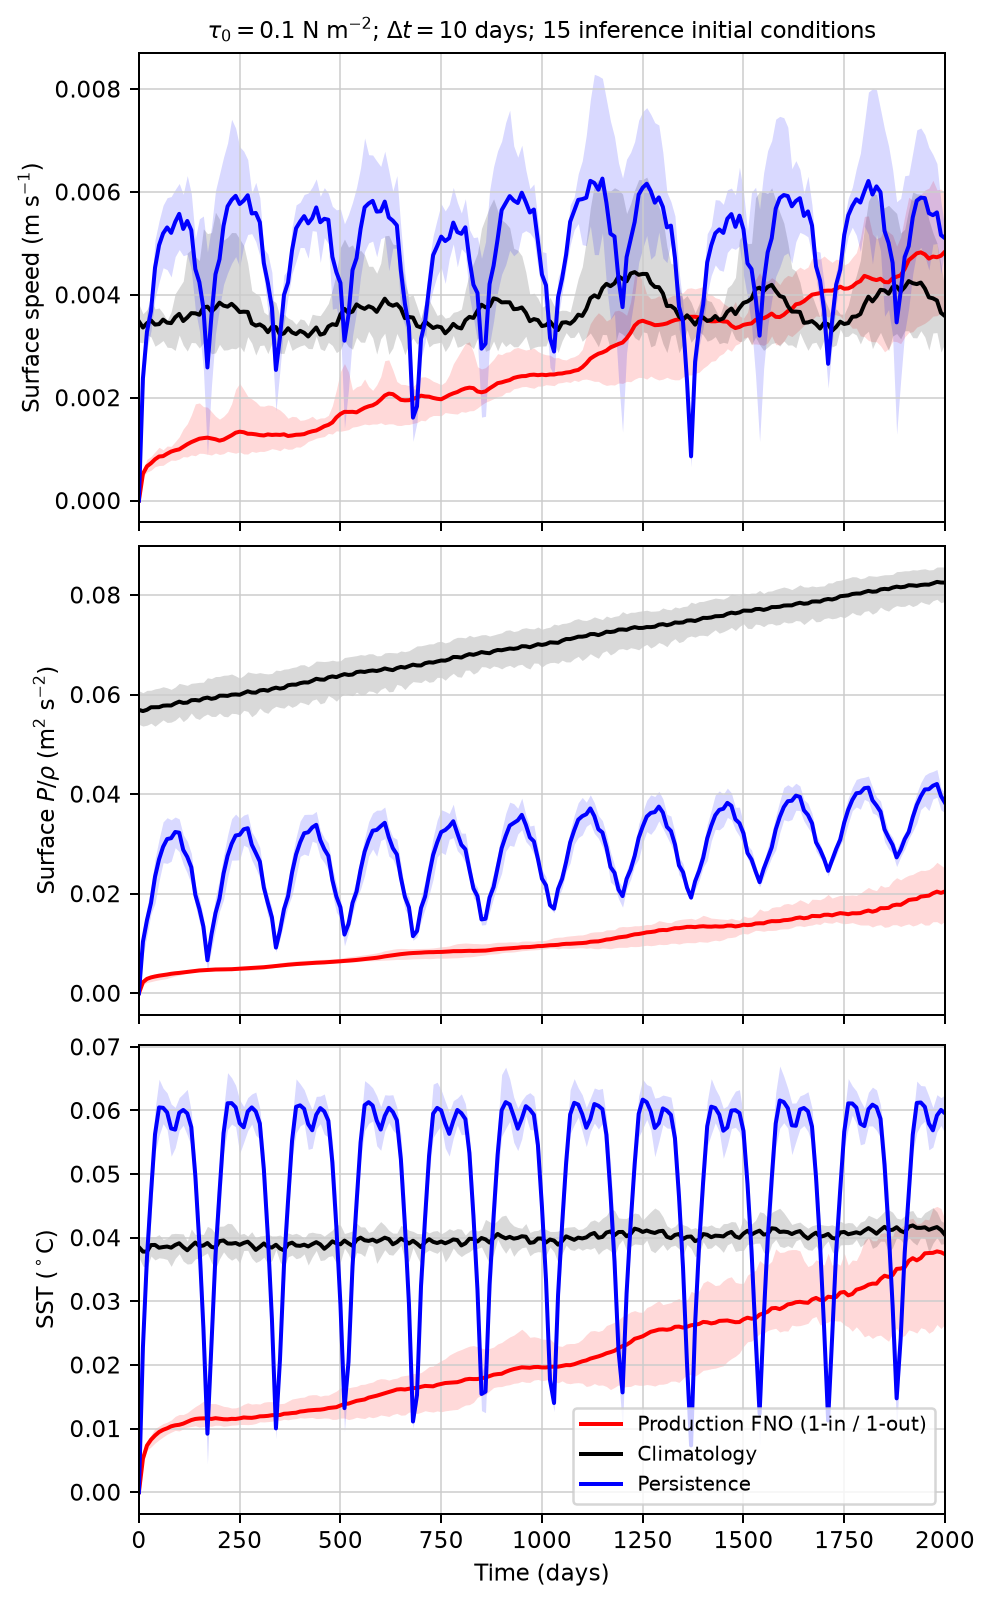
\includegraphics[width=\textwidth]{figures/ft90_figure8_rmse.png}
\caption{Fine-tuned (ft90)}
\end{subfigure}
\caption{Pooled 15-member held-inference RMSE against \MITgcm{} truth,
$\Delta t=10$~d, days 0--2{,}000, S0. The fine-tune's error grows more slowly in
all three fields but has not plateaued by day 2{,}000.}
\label{fig:fig8}
\end{figure}

\begin{figure}[htbp]
\centering
\begin{subfigure}[t]{0.82\textwidth}
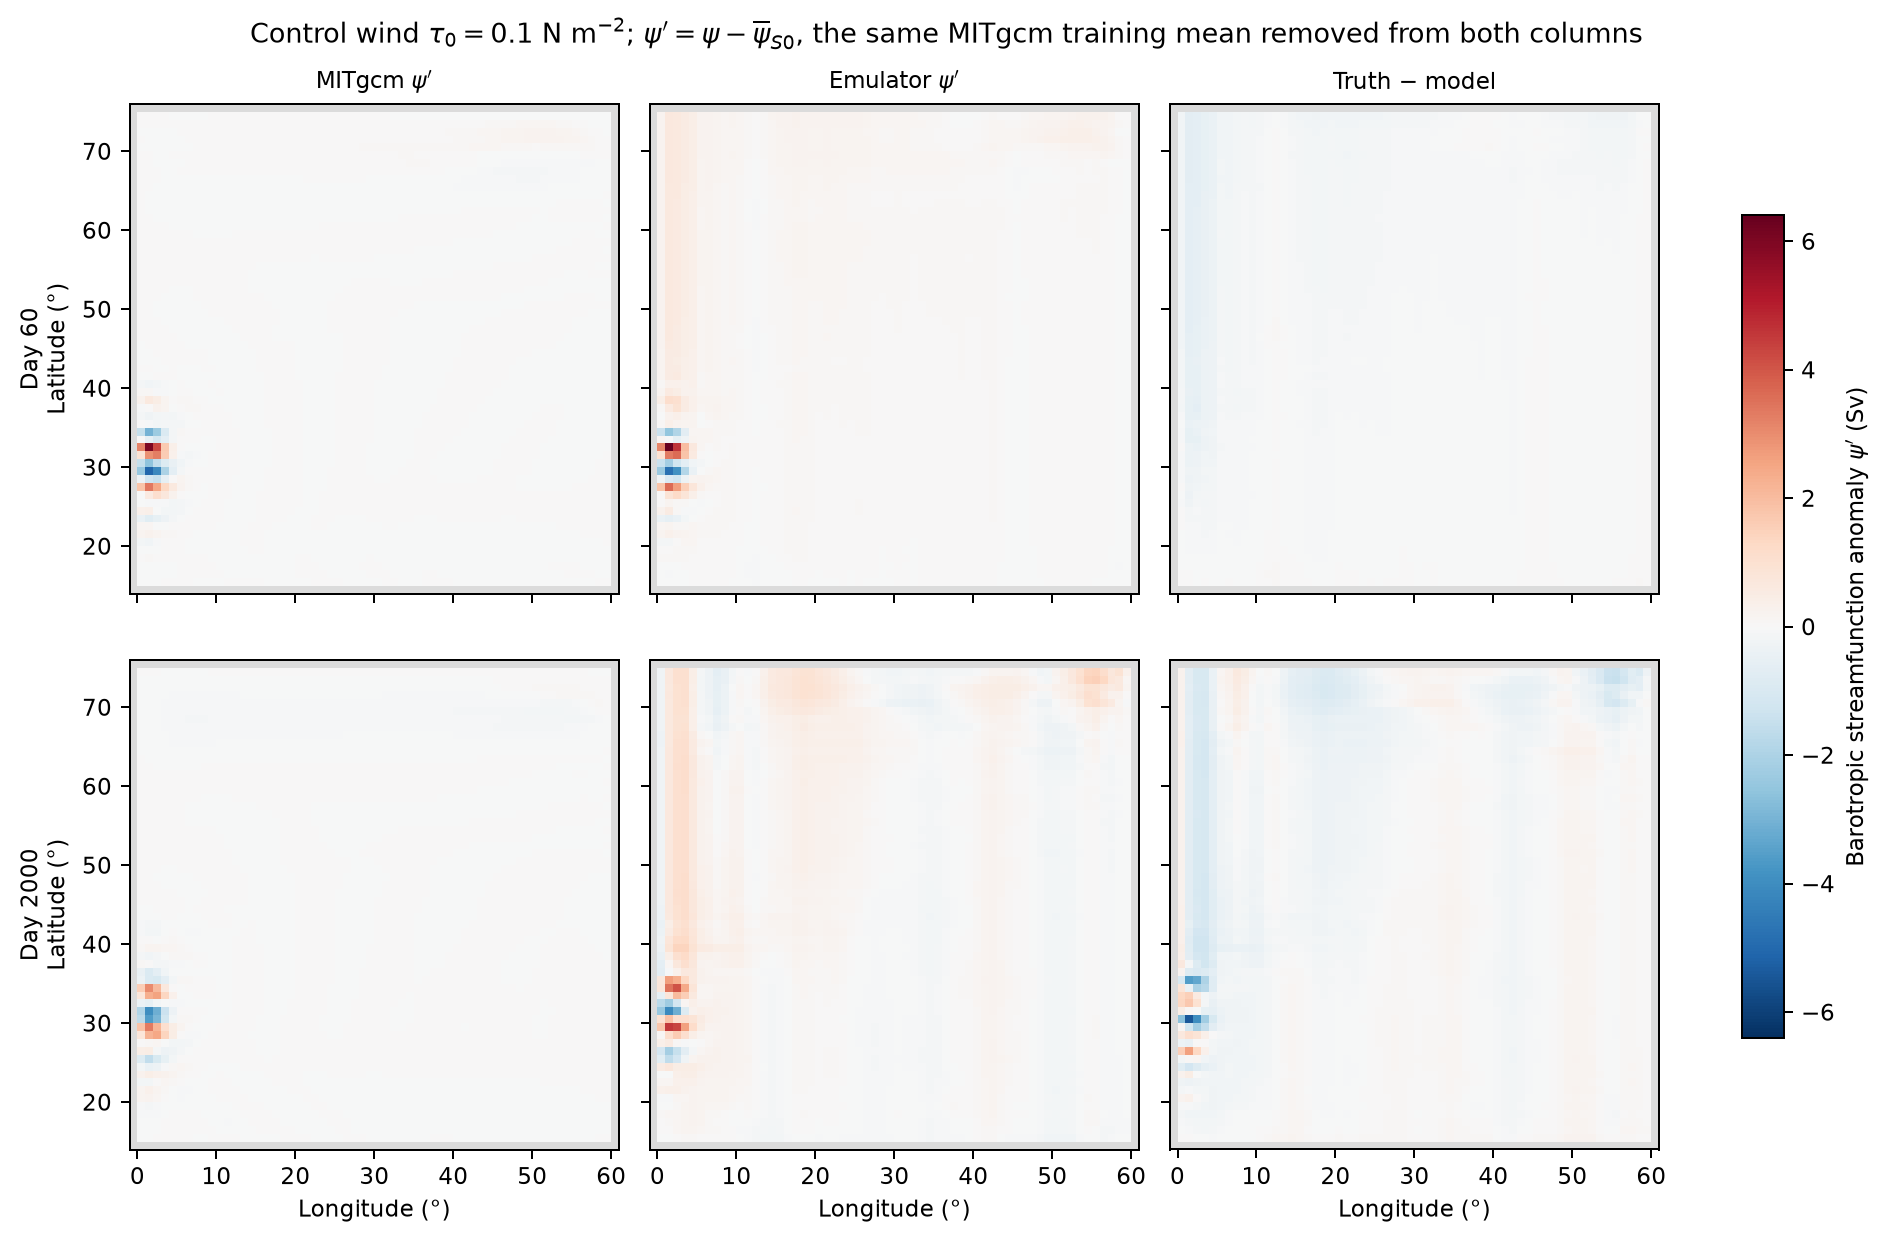
\includegraphics[width=\textwidth]{figures/parent_figure7a_anomaly.png}
\caption{Parent}
\end{subfigure}
\par\smallskip
\begin{subfigure}[t]{0.82\textwidth}
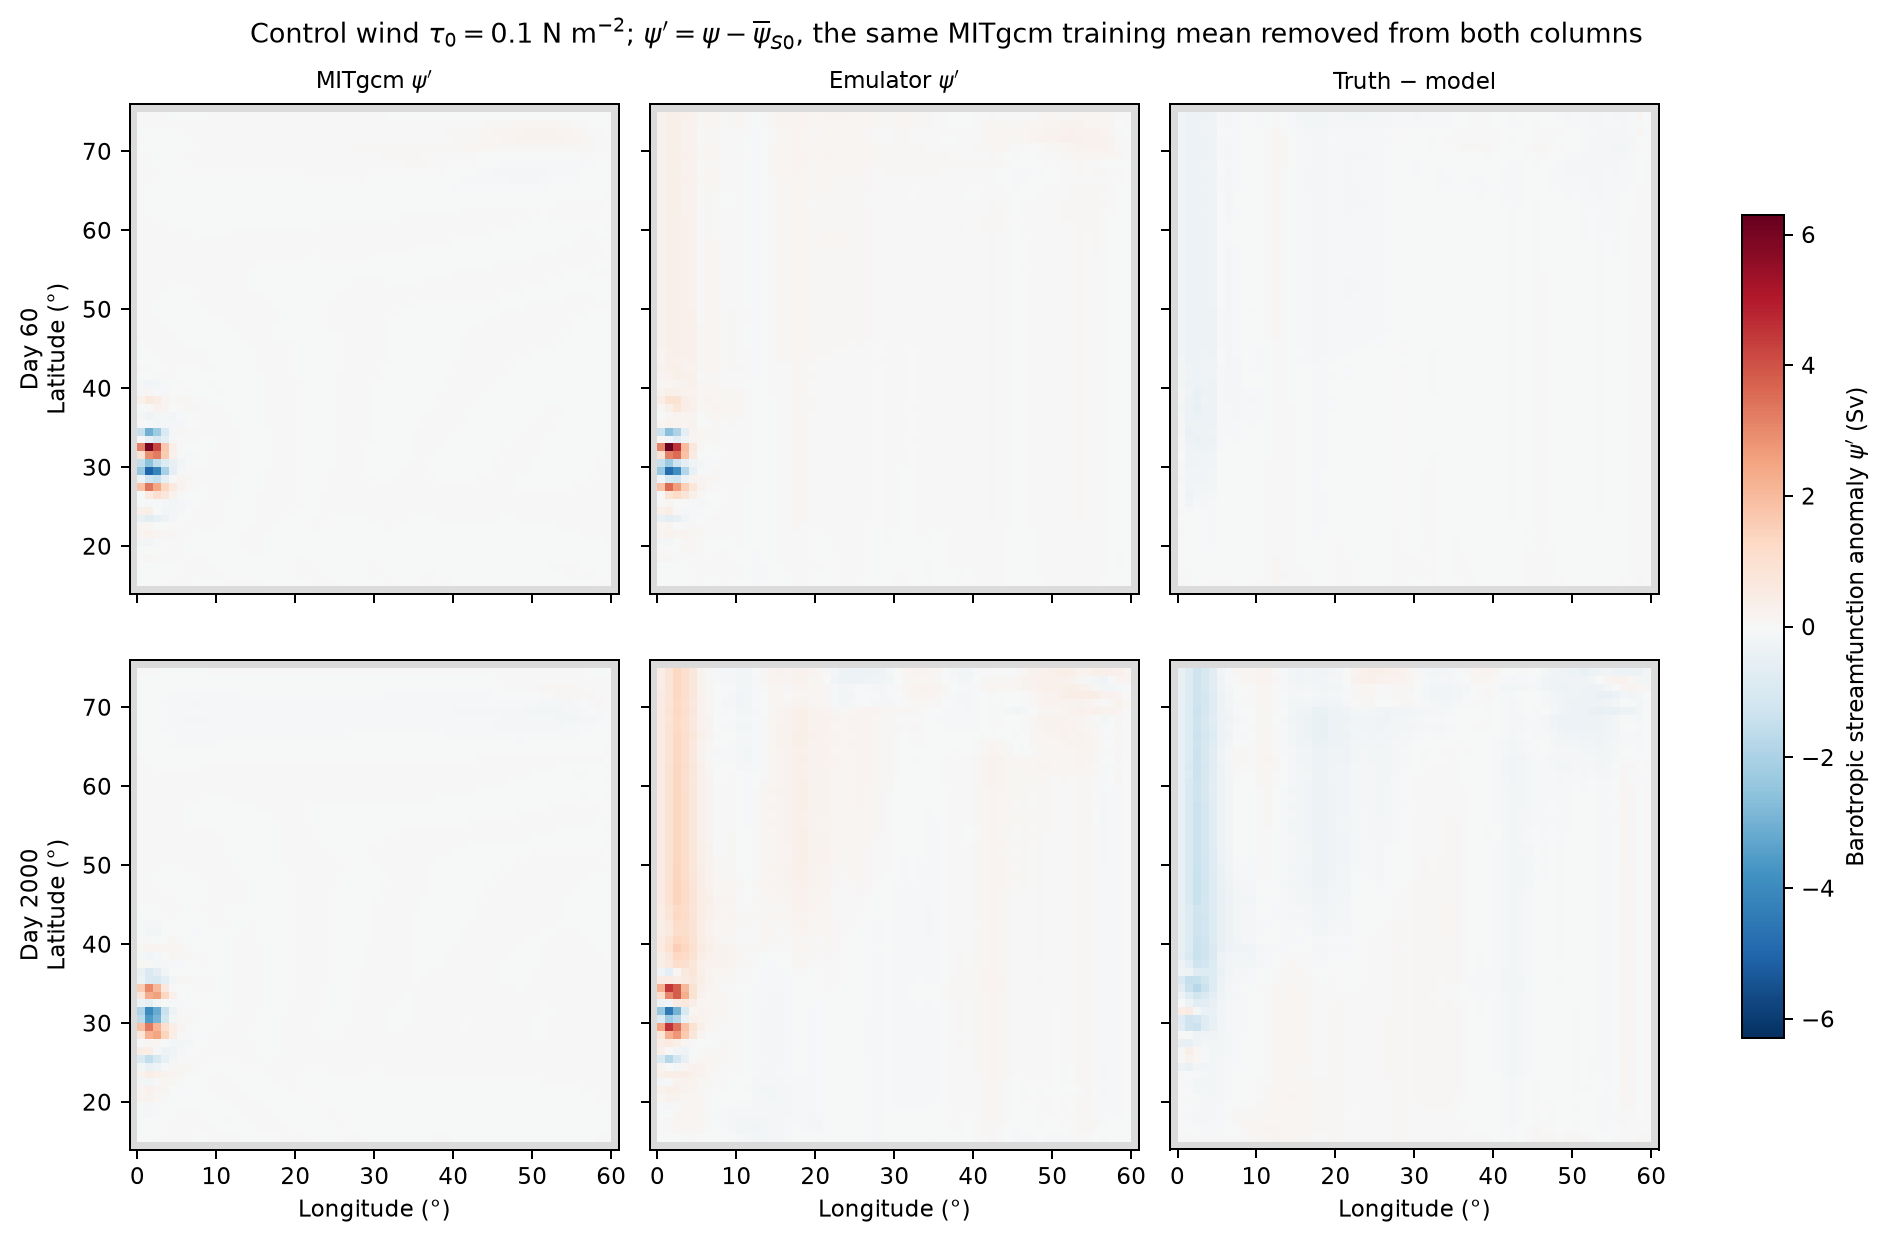
\includegraphics[width=\textwidth]{figures/ft90_figure7a_anomaly.png}
\caption{Fine-tuned (ft90)}
\end{subfigure}
\caption{Barotropic streamfunction anomaly about the training-mean circulation,
day 60 and day 2{,}000, S0. Both models keep the gyre identifiable with a sharp
western boundary current at day 2{,}000; transient amplitude remains
$\sim$1.7--1.8$\times$ too large relative to truth in both.}
\label{fig:fig7a}
\end{figure}

\section{Why a weakly turbulent double gyre}
\label{sec:s0}

All results above use the S0 regime, the control wind amplitude
($\tau_0=0.100$~N\,m$^{-2}$) matching Bire et al.'s~\cite{Bire2025} original
configuration; S1 and S2 are a weaker and a stronger wind perturbation
(0.075 and 0.125~N\,m$^{-2}$). A weakly
turbulent double gyre minimizes chaotic and multiscale complexity, which
gives a clean benchmark to isolate whether the \FNO{} has learned the correct
tangent and adjoint dynamics before moving to a harder, genuinely eddying
regime. Figure~\ref{fig:twin} supports this directly: two \MITgcm{} pickups
differing by a $10^{-3}$ relative perturbation never separate from each
other over 25 simulated years, sitting three to four decades \emph{below} the
control trajectory's own decadal drift throughout. S0 does not exhibit
butterfly-effect sensitivity to initial conditions at this amplitude, so a
discrepancy between the emulator and truth over a long rollout is model error,
not chaotic divergence being amplified — exactly the property needed to make a
Jacobian/adjoint comparison interpretable before repeating it on the
genuinely turbulent 0.25\textdegree{} S0/S1/S2 campaign.

\begin{figure}[htbp]
\centering
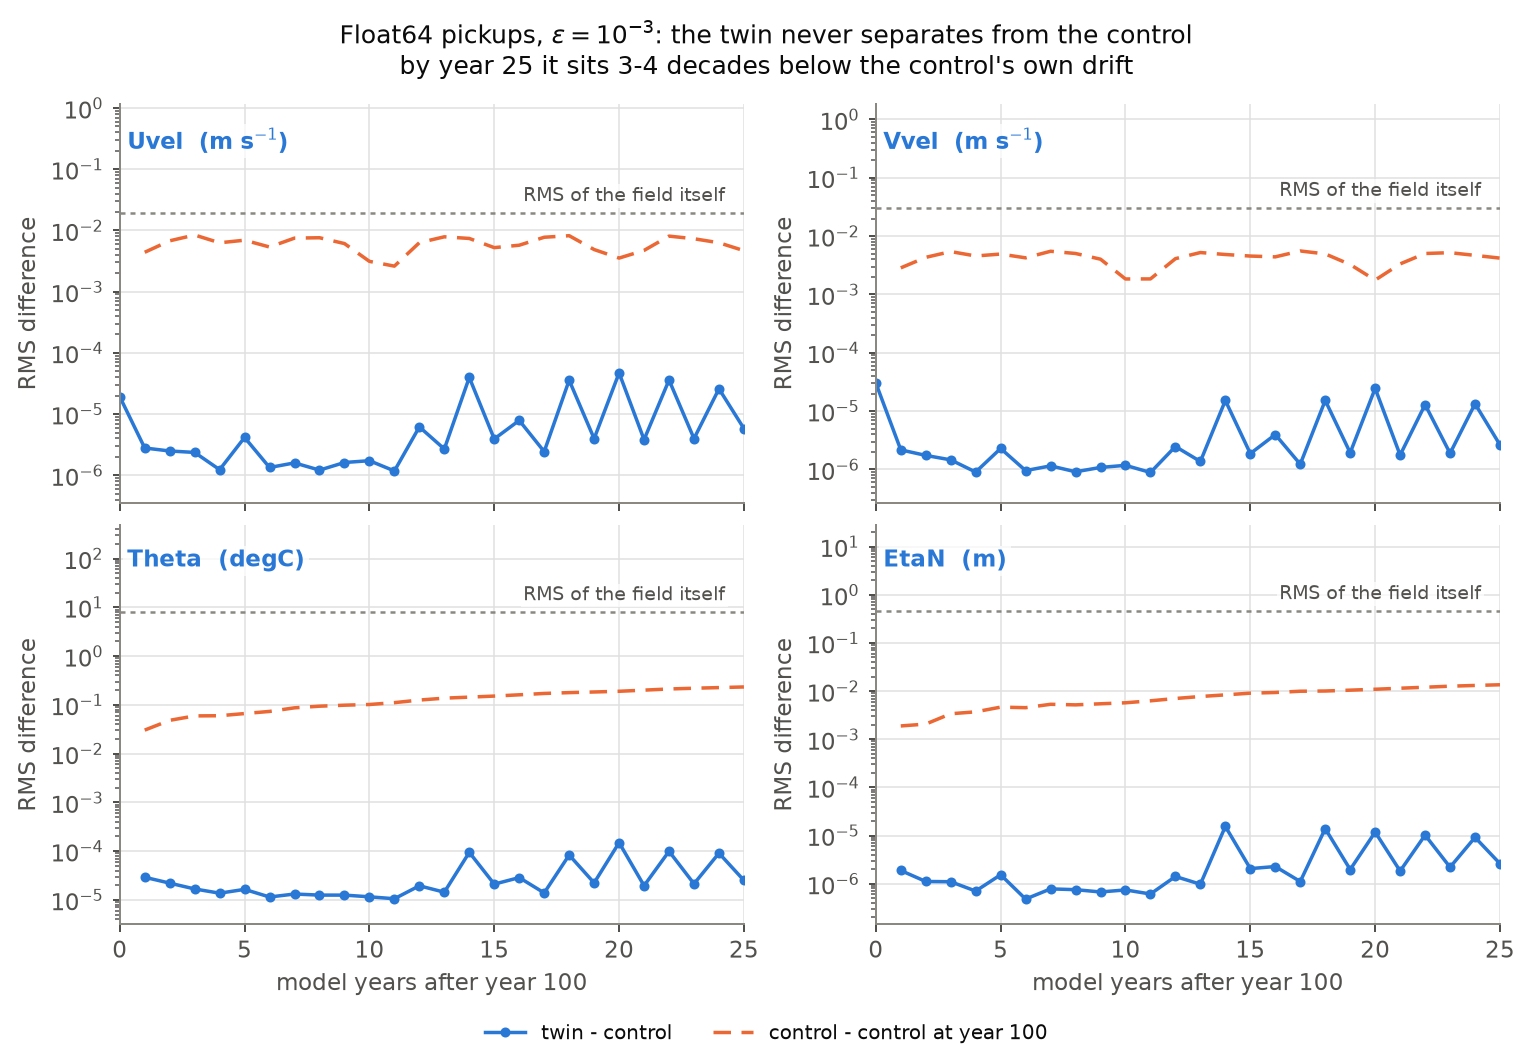
\includegraphics[width=0.85\textwidth]{figures/s0_twin_divergence.png}
\caption{Twin-pickup divergence in S0: RMS difference between a control
trajectory and a $\varepsilon=10^{-3}$ perturbed twin, both float64 \MITgcm{},
over 25 model years. The twin--control difference (solid) never approaches the
control's own year-to-year drift (dashed) or the field's own RMS (dotted),
confirming S0 is not chaotic at this perturbation scale.}
\label{fig:twin}
\end{figure}

\section{Preliminary adjoint study}
\label{sec:adjoint}

\subsection{Objective and setup}

The comparison targets a scalar sea-surface-height objective and its gradient
with respect to the initial surface,
\[
S_T[j,i] \;=\; \frac{\partial J_T}{\partial \eta(j,i,\,t_0)}, \qquad
T\in\{10,20,30,90\}\text{ days},
\]
evaluated two ways on the identical S0 trajectory and window: through
\MITgcm{} differentiated by TAF~6.8.11 (reference, $\sim$20 min per lead), and
through reverse-mode automatic differentiation of the trained, one-input
production \FNO{} (test, seconds). The primary objective is a point functional
at a fixed western-boundary cell $p^\star$, referenced to the domain-mean:
\[
J_{\mathrm{point}} = \eta(p^\star,T) - \langle\eta(T)\rangle_A,
\]
with a secondary five-point meridional Gaussian-smoothed variant,
$J_{\mathrm{kernel}}$, used as a robustness check. Before any comparison
number below is trusted, both producers of $S_T$ are independently verified.
The \MITgcm{}/TAF gradient is checked against direct finite differences of
the forward model over a spread of perturbation sizes, confirming an interior
error minimum rather than a monotonic trend against either round-off or
truncation error; it is exactly reproducible run to run, exactly zero at
every land cell, and reproduces the analytically known conservation of the
basin-mean sea level. The \FNO{}'s reverse-mode gradient is checked against
forward-mode automatic differentiation of the same network, against direct
finite differences of the trained operator itself, and confirmed to satisfy
the adjoint identity $\langle v,Ju\rangle=\langle J^{T}v,u\rangle$ to near
machine precision. Both sides pass every one of these checks at every lead
before any \MITgcm{}-versus-\FNO{} comparison below is reported.

\subsection{Headline result}

The comparison, run against the fine-tuned child (the frozen parent has not yet
been passed through the current pipeline), finds that forecast skill and
adjoint fidelity are not the same thing. Pattern correlation between the
emulator's and \MITgcm{}'s sensitivity maps is essentially zero at every lead
(0.06, $-0.01$, 0.01, 0.02 at 10/20/30/90 days), and the emulator's amplitude is
wrong by a factor of 38 at 10 days, decaying to 6.6 at 90 days
(Figure~\ref{fig:adjoint_curves}). The spatial mismatch is qualitative, not a
fine-scale correction on an otherwise-correct field: at 90 days the true
sensitivity is smooth and concentrated near the western boundary, while the
emulator's is fine-grained and sign-incoherent over most of the basin
(Figure~\ref{fig:adjoint_lead090}). The sensitivity values themselves are
small in an absolute sense --- $O(10^{-5})$ in Figure~\ref{fig:adjoint_lead090}
--- because $S_T$ is a dimensionless influence coefficient: the fraction of a
unit perturbation at one grid cell that survives at the single
objective cell $T$ days later. That influence is spread over the domain's
$\sim$3{,}600 wet cells, so no individual cell is expected to carry an
$O(1)$ share; values several orders below one are the physically expected
scale here, not evidence of a weak or unreliable signal. The emulator also
destroys the analytically conserved basin-mean SSH mode, whose exact answer
is amplitude ratio 1.0 at every lead: the emulator recovers 41\% of it at 10
days and 0.6\% at 90 days.

Two variants of the emulator's sensitivity separate where the error comes
from. $S_{\mathrm{forced}}$ linearizes the emulator about the true \MITgcm{}
trajectory at every ten-day step, so it isolates whether the emulator's own
ten-day Jacobian is right, independent of where its autoregressive rollout
would actually have gone; $S_{\mathrm{free}}$ instead linearizes about the
emulator's own autoregressive trajectory, which is what an operational user
of the deployed model actually gets. The two agree closely --- pattern
correlation 0.996 at 90 days (Figure~\ref{fig:adjoint_curves}) --- so the
mismatch against \MITgcm{} is overwhelmingly Jacobian error rather than
trajectory drift: the emulator's forecast trajectory is close to correct, but
its local derivative along that trajectory is not. That is encouraging for
the training intervention in Section~\ref{sec:plan}, since it means the
quantity that intervention directly supervises is the one that is wrong.

\begin{figure}[htbp]
\centering
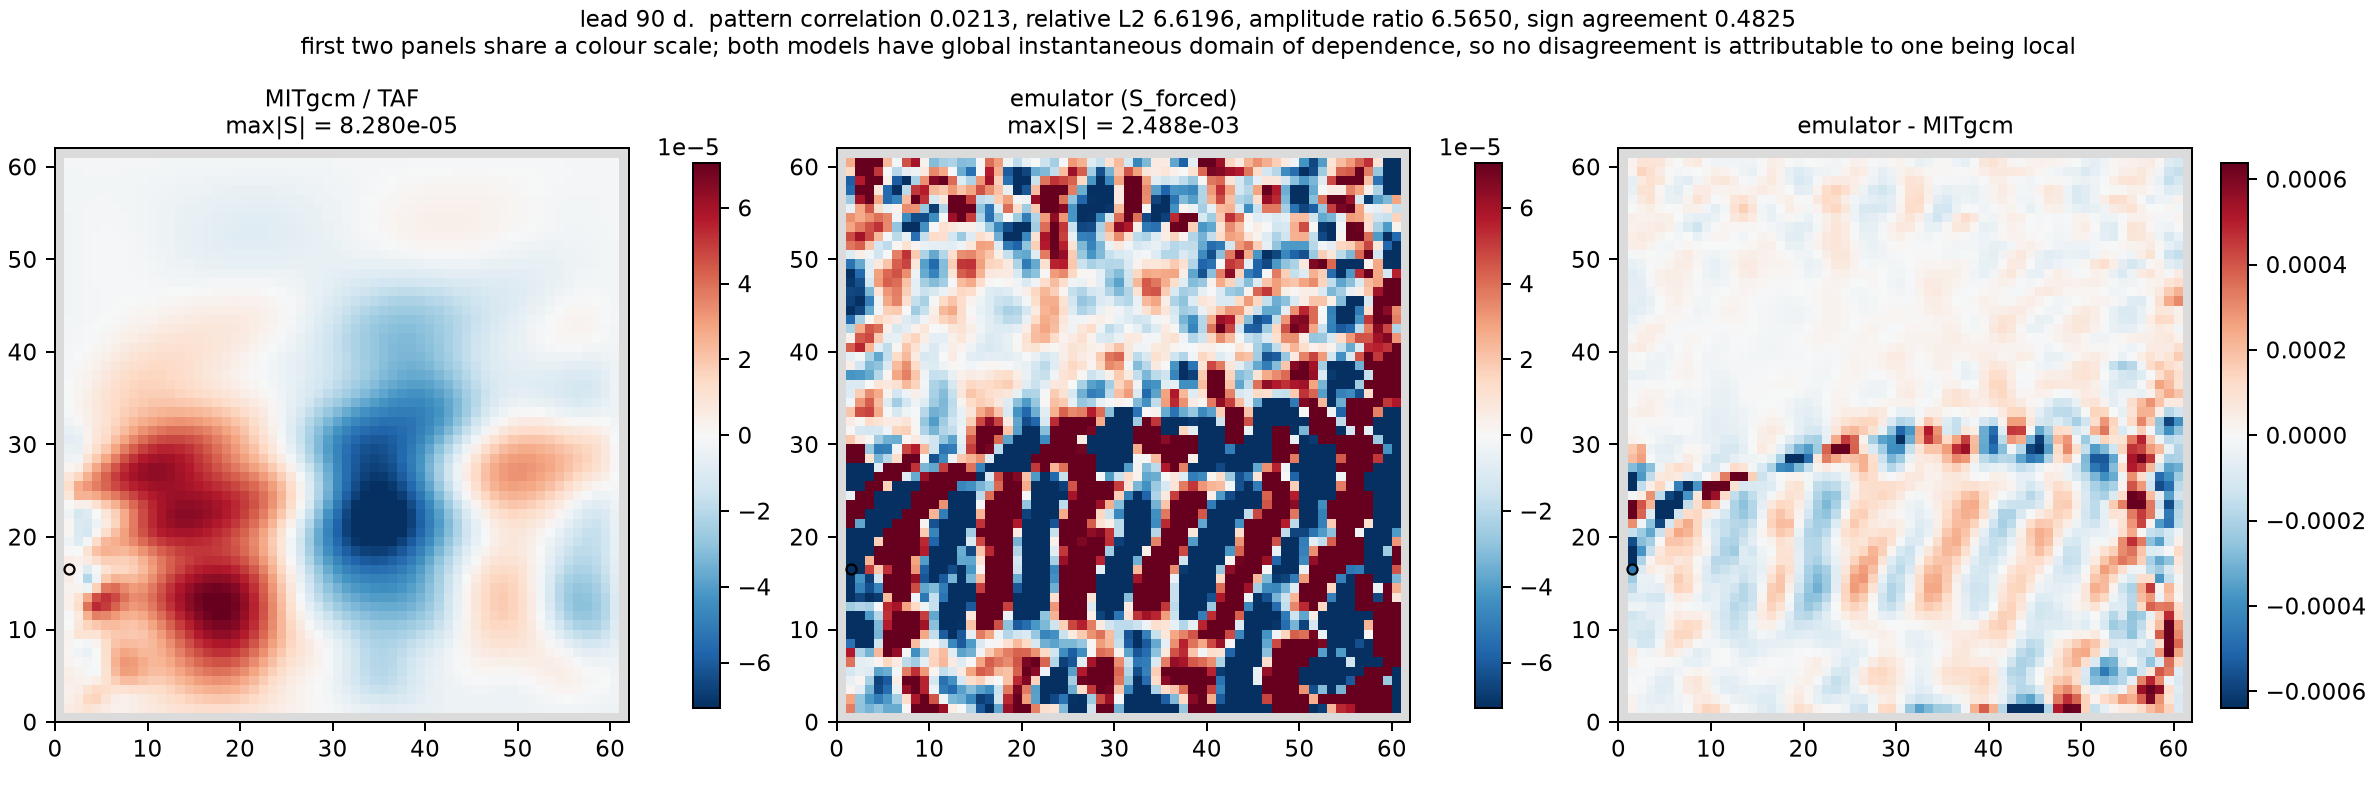
\includegraphics[width=\textwidth]{figures/adjoint_lead090.png}
\caption{Sensitivity map $S_{90}$ at 90 days: \MITgcm{}/TAF (left), the
fine-tuned \FNO{} (centre), and their difference (right), same color scale on
the first two panels. Pattern correlation 0.021, amplitude ratio 6.57.}
\label{fig:adjoint_lead090}
\end{figure}

\begin{figure}[htbp]
\centering
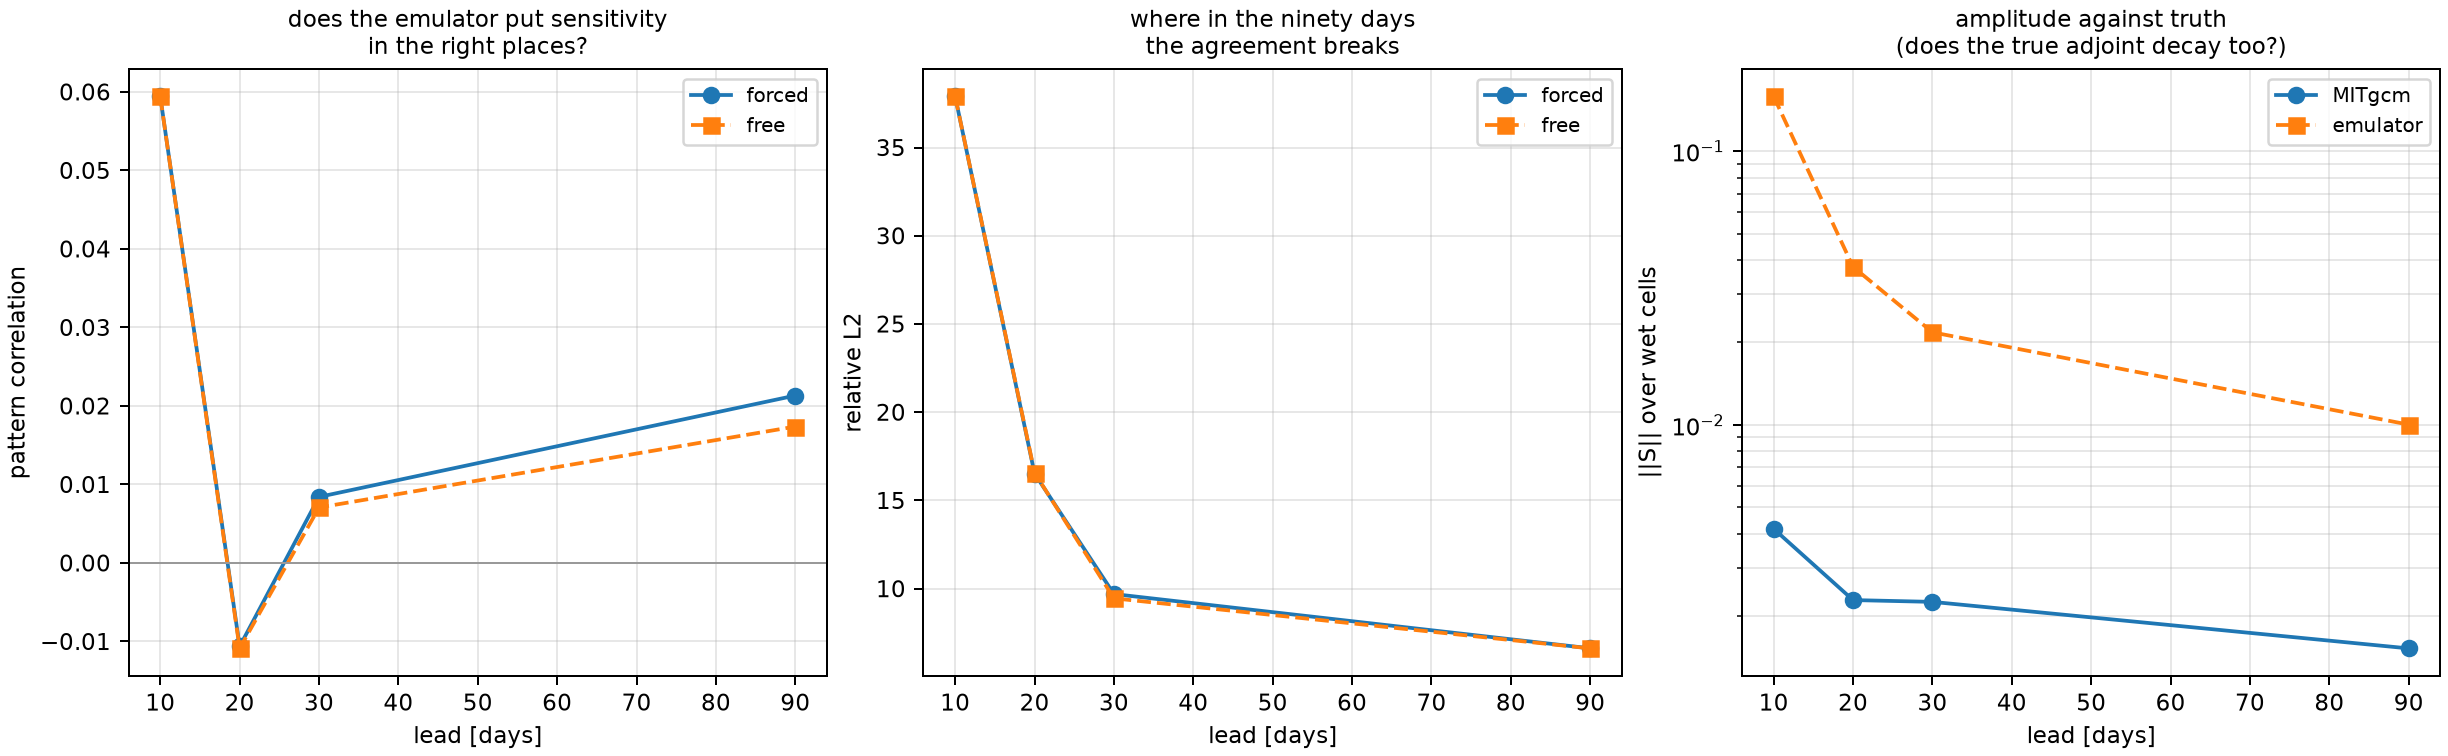
\includegraphics[width=\textwidth]{figures/adjoint_metric_curves.png}
\caption{Lead sweep of the point-objective comparison. Left: pattern
correlation of $S_{\mathrm{forced}}$ and $S_{\mathrm{free}}$ (defined in the
text) against \MITgcm{}, both near zero beyond lead 10. Centre: relative
$L_2$ error, decaying with lead but never small. Right: sensitivity amplitude
against truth --- the \MITgcm{} adjoint decays gently while the emulator's
over-damps by an order of magnitude by day 90.}
\label{fig:adjoint_curves}
\end{figure}

\section{Overview of the adjoint-faithful response training plan}
\label{sec:plan}

The forward-skill/adjoint-fidelity gap in Section~\ref{sec:adjoint} motivates a
targeted intervention: supervise the \FNO{} on finite-difference
directional derivatives of the true \MITgcm{} flow map, without ever letting an
adjoint value influence training or model selection. For a direction $v$ and
amplitude $\epsilon$, the core identity relates forward finite differences to the
Jacobian-vector product,
\[
\frac{M_k(x+\epsilon v) - M_k(x-\epsilon v)}{2\epsilon} = DM_k(x)\,v + O(\epsilon^2),
\]
with the analogous expression for the emulator $F_\theta$. Matching these
forward responses constrains Jacobian-vector products for the sampled
directions; by duality, for any cotangent $w$,
$\langle (DF_k^{T}-DM_k^{T})w,\,v\rangle = \langle w,\,(DF_k-DM_k)v\rangle$,
so a better-matched forward response implies a better-matched adjoint
\emph{projection} onto the sampled direction span, though not the full Jacobian
in unsampled directions --- which is exactly what the blind adjoint test at the
end of the study is designed to check.

\paragraph{The response loss} The intervention is built directly on the
identity above. A large forward-only \MITgcm{} dataset is generated by
integrating paired plus/minus perturbed states: at each sampled anchor state
$x_q$, input group $h(q)\in\{U,V,\Theta,\mathrm{SSH}\}$, direction $v_q$, and
signed amplitude $s\epsilon_q$ with $s\in\{-1,+1\}$, \MITgcm{} is integrated
from $x_q+s\epsilon_q v_q$ and from the unperturbed $x_q$, and the normalized,
signed response
\[
r_{M,q,k}^{s} = \frac{\mathcal N\bigl[M_k(x_q+s\epsilon_q v_q)\bigr]-\mathcal N\bigl[M_k(x_q)\bigr]}{s\epsilon_q}
\]
is recorded at each ten-day lead $k$ out to a role-dependent horizon, in the
same pointwise-normalized coordinates $\mathcal N(\cdot)$ the emulator is
trained in. The analogous quantity $r_{F,q,k}^{s}$ is computed from the
emulator on the same edited initial states. A new model, $F_\theta'$, is
trained from random initialization with the same architecture, data split,
optimizer schedule, and eight-term forward objective $L_{\mathrm{nominal}}$ as
the production emulator of Section~\ref{sec:emulator}, plus exactly one
additional term added on a predeclared subset of optimizer steps,
\[
L_{\mathrm{total}} = L_{\mathrm{nominal}} + \lambda_{\mathrm{resp}}\,L_{\mathrm{response}}.
\]
Writing $g\in\{U,V,\Theta,\mathrm{SSH}\}$ for an output group and
$d_{h,g,k}^2$ for the response-training-data mean-square response of output
group $g$ to a perturbation of input group $h$ at lead $k$,
\[
L_{\mathrm{response}} = \operatorname{mean}_{q}\;\frac{1}{8}\sum_{s\in\{-1,+1\}}\sum_{g}
\frac{\operatorname{mean}_{c\in g,\,\mathrm{wet}}\bigl(r_{F,q,k}^{s}-r_{M,q,k}^{s}\bigr)^2}{d_{h(q),g,k}^2},
\]
averaged over the sampled directions $q$ and, for the subset of directions
extended beyond ten days, over lead $k$ as well. Dividing by $d_{h,g,k}^2$
puts every input/output pair on a comparable, unitless scale regardless of
its physical units or channel count, so no single group can dominate the
loss simply by having larger natural units or more vertical levels. No
ordinary state loss is placed on the perturbed trajectories themselves --- the
signed response is the only quantity supervised --- and no adjoint output of
any kind, from \MITgcm{}/TAF or from the emulator, enters $L_{\mathrm{response}}$
or any other part of training: the response term is the only difference
between this model and the existing production training recipe.

\paragraph{Data scale} Generating this dataset is itself a substantial
\MITgcm{} campaign. Perturbing $U$, $V$, $\Theta$, and sea-surface height at
many spatial locations and times across the three wind regimes, both signs,
mostly to a ten-day lead with a smaller subset carried to 60 or 90 days,
totals 57{,}750 model-days (160.4 model-years) of forward-only integration
across the training, validation, and a held-out blind set. As above, no
\MITgcm{} adjoint or TAF output is used anywhere in generating this data or
in training: every quantity feeding $L_{\mathrm{response}}$ comes from
ordinary forward integrations.

\paragraph{Direction and status} The plan is staged so that every design
choice --- how large a perturbation to use, how to weight the response term,
which checkpoint to keep --- is frozen using forward evidence alone, before
the trained model is ever compared against \MITgcm{}'s adjoint. Concretely:
first calibrate, with a small forward-only pilot, how large a perturbation
can be while the response still behaves linearly; then generate the full
training/validation/blind response dataset at that calibrated amplitude;
then train the new model, choosing its response weight and checkpoint using
only forward-forecast skill and held-out response error, while requiring it
to match the existing production emulator's ordinary forecast performance;
and only once all of that is locked in, evaluate the trained model's adjoint
against \MITgcm{}/TAF as in Section~\ref{sec:adjoint}, to see whether
forward-response supervision closes the gap found there. This ordering is
deliberate: it means a good- or bad-looking adjoint result can never feed
back into how the model was built or chosen.


\section*{Next steps}

The immediate next step is a small forward-only pilot that perturbs each of
$U$, $V$, $\Theta$, and sea-surface height at a handful of locations and
candidate amplitudes, to fix one amplitude per variable before large-scale
data generation begins. From there the plan moves to generating the full
response dataset, training the response-aware model and choosing its
response weight, and finally revisiting the Section~\ref{sec:adjoint}
comparison against \MITgcm{}/TAF with the new model, to test whether this
forward-only supervision is enough to fix what Section~\ref{sec:adjoint}
found.

\bibliographystyle{elsarticle-num}
\bibliography{references}

\end{document}
